\documentclass[aspectratio=169]{beamer}
\usetheme{Bruno}

\usepackage{graphicx}
\usepackage{subcaption}
\usepackage{mwe}
\usepackage{multicol}
\usepackage{amsmath}
\usepackage{algorithm}
\usepackage[noend]{algpseudocode}
\usepackage{float}

%------------------------------------------------------------
%The next block of commands puts the table of contents at the 
%beginning of each section and highlights the current section:

\AtBeginSection[]
{
  \begin{frame}
    \frametitle{Table of Contents}
    \tableofcontents[currentsection]
  \end{frame}
}
%------------------------------------------------------------

\title{Artificial Intelligence in Train Scheduling Problems}
\author{
    Kieran Molloy
}
\institute{Manchester Metropolitan University}
\date{\today}
\background{assets/.Global/asd.jpg}

\begin{document}

\maketitle

\begin{frame}{Table of Contents}
    \tableofcontents
\end{frame}

\begin{frame}{Project Motivation}
    Optimisation of train networks can provide return on all optimality factors; profit, timeliness or robustness. Train networks provide a unique problem where infrastructure expansions are complicated, expensive and disruptive. This leads to largely scheduling based problems, which this project is based upon.
\end{frame}

\begin{frame}{Brief Introduction}
    %The project can be split into the below sections, each section can be used on its own, but are more cohesive in order.
    \begin{figure}
        \centering
        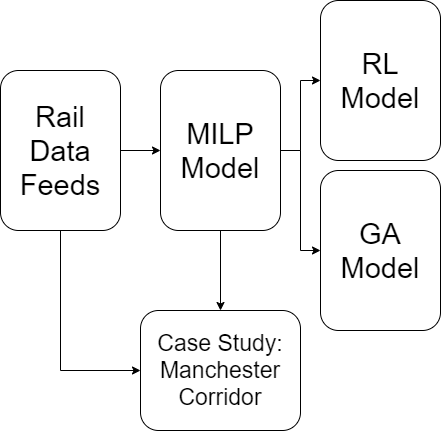
\includegraphics[height=14em]{assets/Introduction/project-outline.png}
        \caption{Project Outline}
        \label{fig:project-outline}
    \end{figure}
\end{frame}

\begin{frame}{Brief Introduction}
    %The project may seem disjointed, however this is due to the original plan looked like this
    \begin{figure}
        \centering
        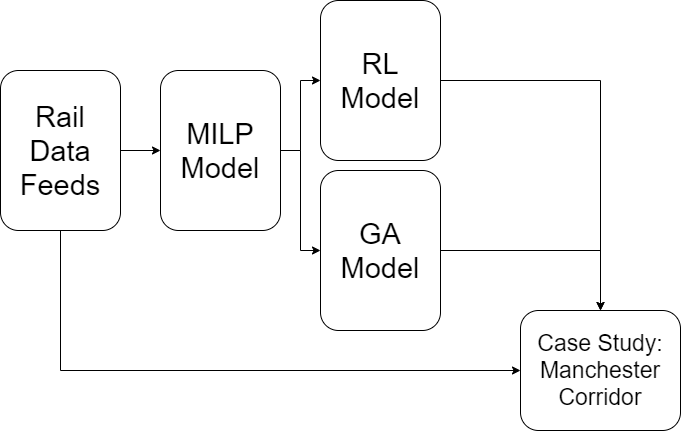
\includegraphics[height=14em]{assets/Introduction/desired-project-outline.png}
        \caption{Intended Project Outline}
        \label{fig:i-project-outline}
    \end{figure}
\end{frame}



%------------------------------------------------------------------------------------------
% RDF
\section{Rail Data Feeds}
%------------------------------------------------------------------------------------------

\begin{frame}{RDF - Implementation}
    %The project may seem disjointed, however this is due to the original plan looked like this
    \begin{figure}
        \centering
        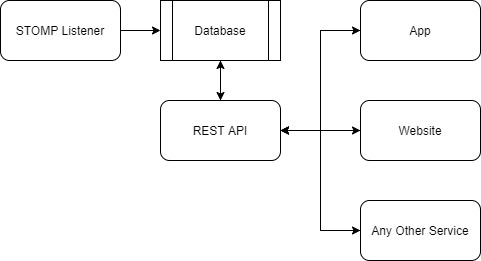
\includegraphics[width=0.60\textwidth]{assets/RDF/rdf-flow.jpg}
        \caption{Rail Data Feeds Program Flow}
        \label{fig:rdf-flow}
    \end{figure}
\end{frame}

\begin{frame}{RDF - Purpose}
    %
    \begin{itemize}
        \item View the Network Live
        \item Save Network Statistics
        \item Create Real World Test Sets
    \end{itemize}
\end{frame}

\begin{frame}{RDF - Outcomes}
    %
    \begin{itemize}
        \item Network Rail Listener
        \item Huxley Connector
        \item Network Rail Historic Database
        \item REST API
        \item Website 
    \end{itemize}
\end{frame}

%------------------------------------------------------------------------------------------
% MILP
\section{Mixed Integer Linear Programming}
%------------------------------------------------------------------------------------------

\begin{frame}{MILP Model - TSP}
    % The Basic MILP TSP is extremely well studied, hence not discussed much in this project. It can be summarised using this objective function
    Objective Function
    \begin{equation*}\label{eq:milp-tsp-obj}
        \sum_{n=1}^{N}{A_{n,M}^{s}-D_{n,0}^{s}}
    \end{equation*}
    Example Constraints:
    \begin{align*}
        D_{n,m}^{r} &\leq A_{{n+1},m}^{r} - H \\
        \vspace{1em} \\
        A_{n,{m+1}}^{r} &\geq D_{n,m}^{r}+E_m
    \end{align*}
\end{frame}

\begin{frame}{MILP Model - TRSP}
    % 
    Objective Function
    \begin{equation*}\label{eq:milp-tsp-obj-2}
        \sum_{n=1}^{N}{A_{n,M}^{r} - A_{n,M}^{o}}
    \end{equation*}
    Example Constraints:
    \begin{equation*}
        D_{n,m}^{r} = D_{n,m}^{0} % All trains run on schedule before delay
    \end{equation*}
    \hspace{35pt}$\delta_D > 1, \delta_t < D_{\delta_n}^{\delta_D -1}+E_{\delta_{D}-1}\rightarrow$ \dots
    \begin{equation*}
        A_{\delta_n,\delta_D}^{r} \geq D_{\delta_n,\delta_D -1}^{0} + \delta_d + E_{\delta_d - 1} %If after delay, train will be delayed
    \end{equation*}
\end{frame}

\begin{frame}{MILP Model - TRSP (Passenger Weighted)}
    % 
    Objective Function
    \begin{equation*}\label{eq:milp-tsp-obj-3}
        \sum_{n=1}^{N}{P_{n,M}^{c} A_{n,M}^{r}}
    \end{equation*}
    Example Constraints:
    \begin{align*}
        C-P_{n,{m-1}}^{l} < 100 &\rightarrow P_{c}^{n,m} \leq 20\lambda_{n,m} \\
        C-P_{n,{m-1}}^{l} \geq 100 &\rightarrow P_{c}^{n,m} \leq 50\lambda_{n,m} \\
        P_{n,m}^{c} &\leq D+{n,m}^{r} - 50 A_{n,m}^{r}
    \end{align*}
\end{frame}

\begin{frame}{MILP Model - Outcomes}
    \begin{itemize}
        \item MiniZinc TRSP Standard Model
        \item Series of Associated FlatZinc Data Files
        \item Minizinc TRSP Passenger Weighted Model
        \item Series of Assocaited FlatZinc Data Files
    \end{itemize}
\end{frame}

%------------------------------------------------------------------------------------------
% GA
\section{Genetic Algorithms}
%------------------------------------------------------------------------------------------
\begin{frame}{GA - General Algorithm}
    %
    \begin{algorithmic}
        \State $P \gets$ generatePopulation[100]  \Comment{Get 100 random variables}
        \While{endCondition = false}
            \State $P \gets $ selection($P$)
            \State $P \gets $ crossover($P$)
            \State $P \gets $ mutation($P$)
            \State $B \gets $ fitness($P$)
            \If{B == optimal}
               \State endCondition $\gets$ true
            \EndIf
        \EndWhile
        
        \Return B,P
    \end{algorithmic}
\end{frame}

\begin{frame}{GA - TSP Framework}
    %
    \begin{table}[]
        \begin{tabular}{|l|lll|lll|}
        \hline
                        & \multicolumn{6}{l}{Phenotype}                                          \\
        \hline
                        & toc & line & unit & origin & destination & intermediate                \\
        \hline
        Bit Length      & 2   & 8    & 8    & 12     & 12          & $12n$                       \\
        Representations & 4   & 256  & 256  & 4096   & 4096        & $n(2^{12})$                    \\
        \hline
        \end{tabular}
    \end{table}
\end{frame}

\begin{frame}{GA - Basic Scenario}
    %
    \begin{figure}
        \centering
        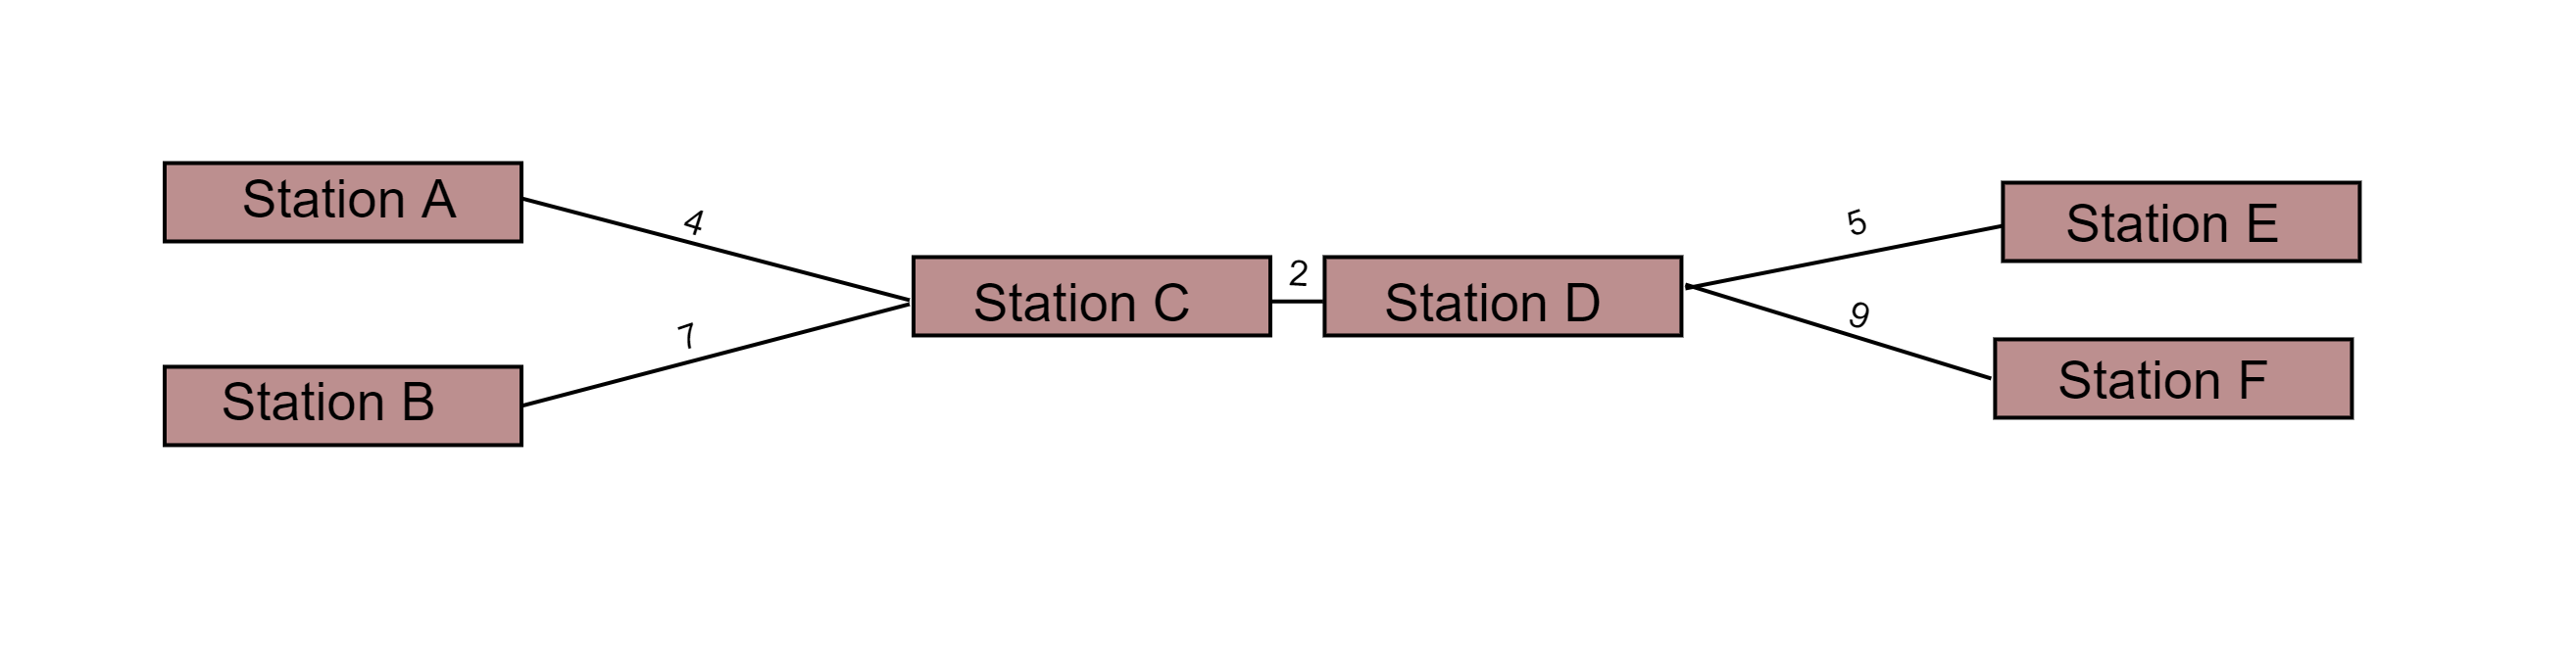
\includegraphics[width=0.60\textwidth]{assets/GA/basicExampleChartCropped.png}
        \caption{Toy Example Map}
        \label{fig:ga-toy}
    \end{figure}
\end{frame}

\begin{frame}{GA - Basic Scenario}
    %
    \begin{figure}
        \centering
        \begin{subfigure}[t]{0.3\textwidth}
            \centering
            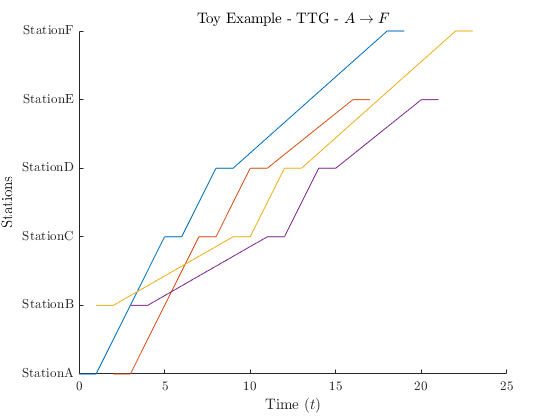
\includegraphics[width=\linewidth]{assets/GA/toy1.png}
            \caption{Stage 1}
            \label{fig:ga-stage1}
        \end{subfigure}
        \begin{subfigure}[t]{0.3\textwidth}
            \centering
            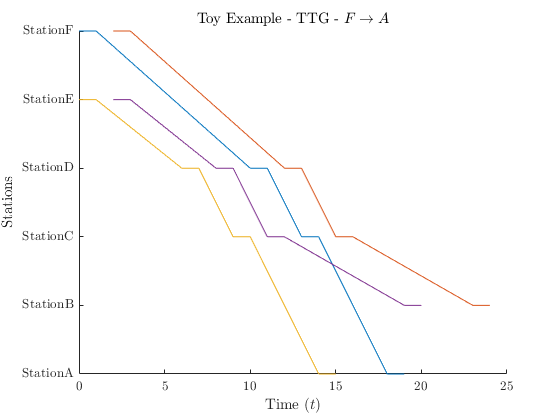
\includegraphics[width=\linewidth]{assets/GA/toy2.png}
            \caption{Stage 2}
            \label{fig:ga-stage2}
        \end{subfigure}
        \begin{subfigure}[t]{0.3\textwidth}
            \centering
            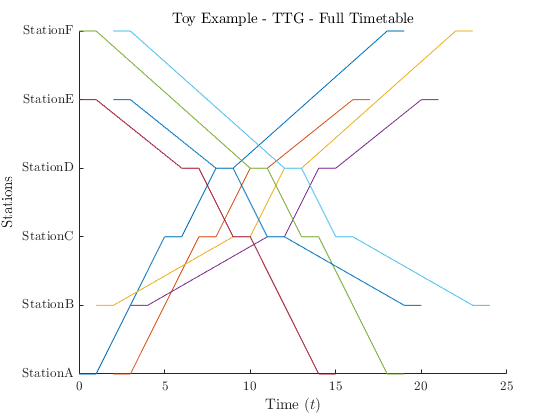
\includegraphics[width=\linewidth]{assets/GA/toy3.png}
            \caption{Stage 3}
            \label{fig:ga-stage3}
        \end{subfigure}
    \end{figure}
\end{frame}

\begin{frame}{GA - Basic Scenario}
    %
    \begin{figure}
        \centering
        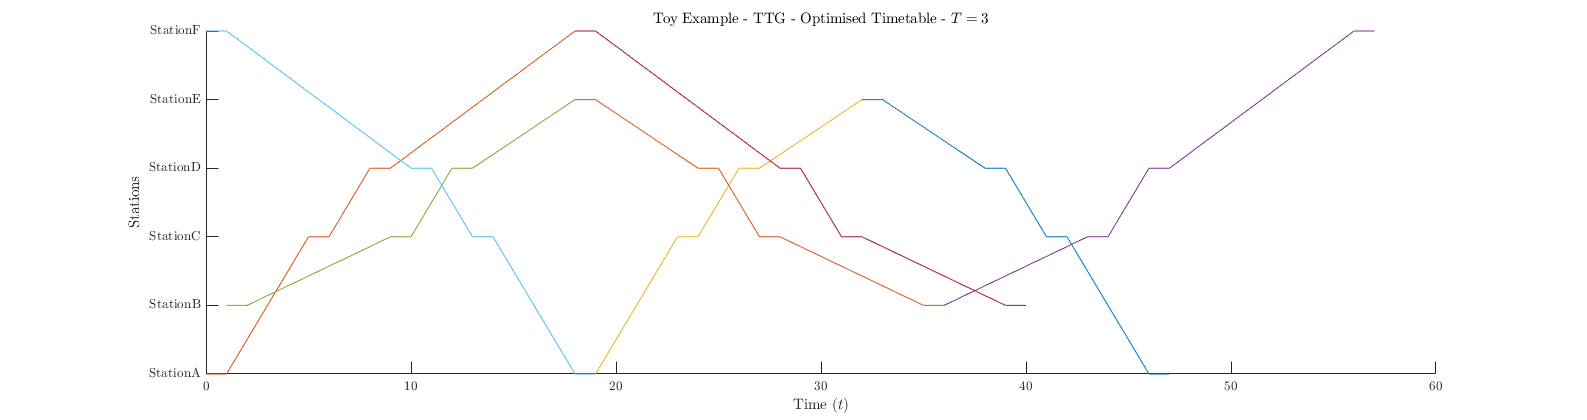
\includegraphics[width=\textwidth]{assets/GA/toy4.png}
        \caption{Toy Example Combined Stages}
        \label{fig:ga-toy-stages}
    \end{figure}
\end{frame}

\begin{frame}{GA - Medium Scenario}
    %
    \begin{figure}
        \centering
        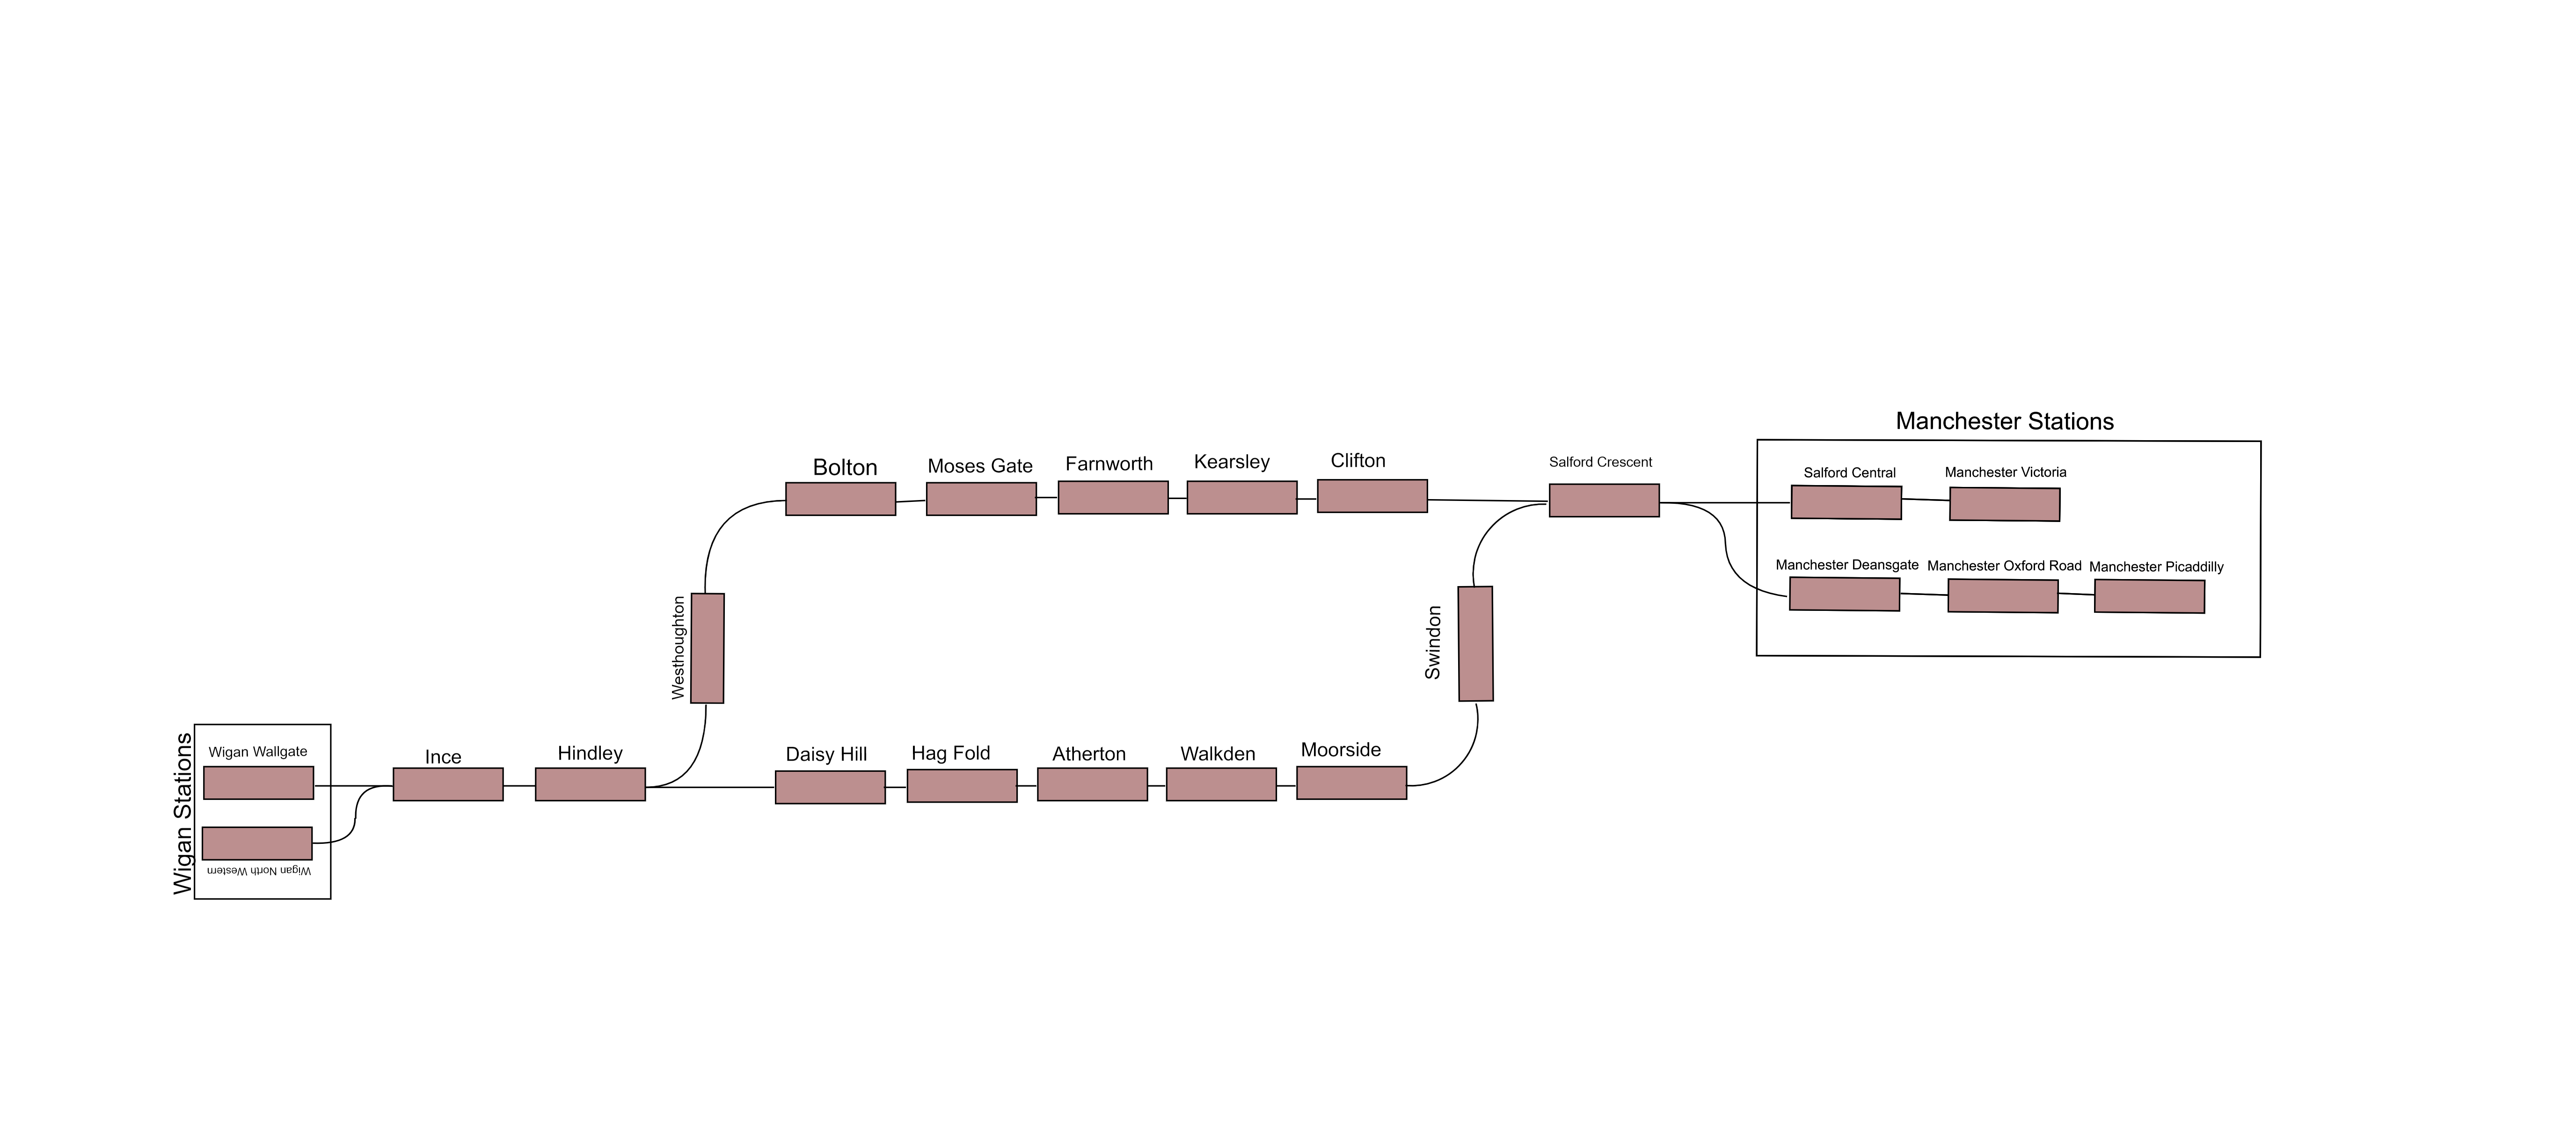
\includegraphics[width=0.9\textwidth]{assets/GA/SmallNetwork.png}
        \caption{Small Example Map}
        \label{fig:ga-small}
    \end{figure}
\end{frame}

%------------------------------------------------------------------------------------------
% RL
\section{Reinforcement Learning}
%------------------------------------------------------------------------------------------
\begin{frame}{SBB Challenge}
    %
    \begin{figure}
        \centering
        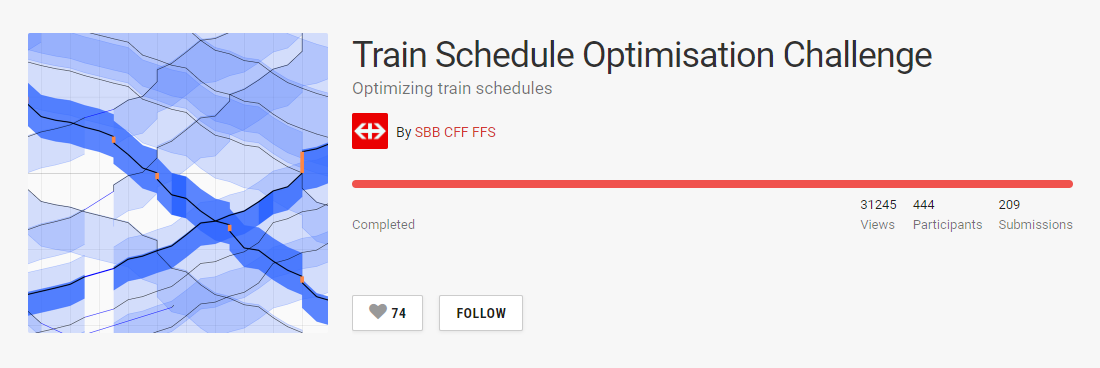
\includegraphics[width=\textwidth]{assets/RL/SBB.PNG}
        \caption{Crowd AI SBB Challenge}
        \label{fig:sbb}
    \end{figure}
\end{frame}

\begin{frame}{SBB Challenge}
    %
    \begin{table}
        \small
        \centering
        \begin{tabular}{|c|c|cc|c|cc|}
            \hline
            ID & Name & Trains & Routing & Difficulty \\
            \hline
            01 & dummy & 4 & V.Few & V.Simple \\
            02 & a\_little\_less\_dummy & 58 & Few & Simple \\
            03 & FWA\_0.125 & 143 & Few & Simple \\
            04 & V1.02\_FWA\_without\_obstruction & 148 & Few & Medium \\
            05 & V1.02\_FWA\_with\_obstruction & 149 & Medium & Medium*\\
            06 & V1.20\_FWA & 365 & High & V.Hard \\
            07 & V1.22\_FWA & 467 & High & V.Hard \\
            08 & V1.30\_FWA & 133 & V.High & V.Hard \\
            09 & ZUE\-ZG\-CH\_0600\-1200& & & 287 & VV.High & VV.Hard \\
            \hline
        \end{tabular}
        \caption{Description of Problem Scenarios}
        \label{tab:all-scenarios}
    \end{table}
\end{frame}



\begin{frame}{RL - Delayed Q-Learning}
    \begin{columns}[T, onlytextwidth]
        \begin{column}{0.5\textwidth}
            Modelling a PACMDP \\
            Update Function\:
            \begin{figure}
                \centering
                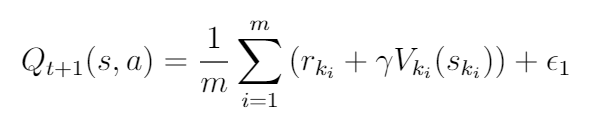
\includegraphics[width=\textwidth]{assets/RL/EQ1.PNG}
            \end{figure}
        \end{column}
        
        \begin{column}{0.5\textwidth}
            \begin{figure}
                \centering
                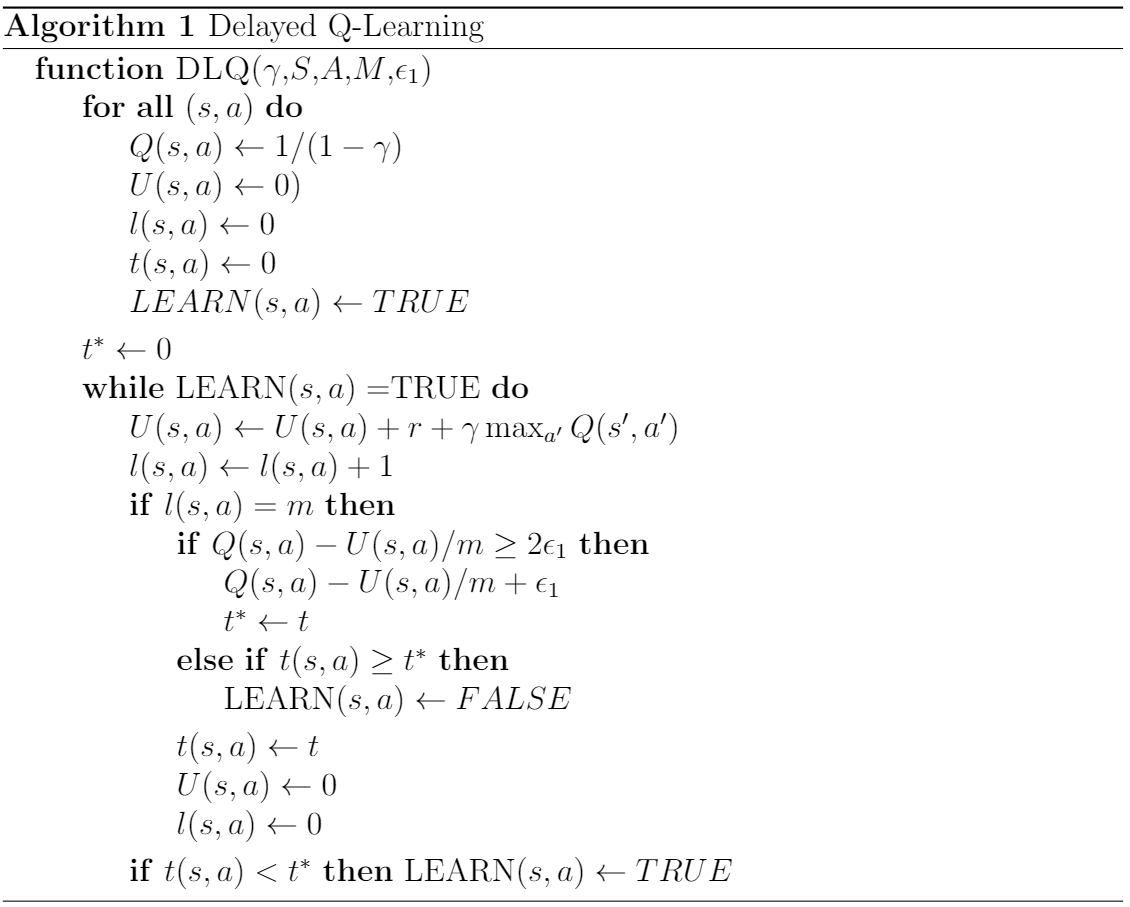
\includegraphics[width=0.7\textwidth]{assets/RL/ALG1.PNG}
                \caption{Delayed Q-Learning}
                \label{fig:dlq}
            \end{figure}
        \end{column}
    \end{columns}
\end{frame}



\begin{frame}{RL SBB - Objective Function}
    % 
    \begin{multline*}\label{eq:rl-obj}
        \frac{1}{60}\times\Bigg[\sum_{\mathcal{S},\mathcal{R},\mathcal{RS}}{weightIn_{rs}\times \max{\bigg(0,\big(t_{s,r,rs}^{entry} - inLat_{s,rs} \big)\bigg)}}\\+weightOut_{rs} \times \max{\bigg(0,\big(t_{s,r,rs}^{exit} - outLat_{s,rs}\big)\bigg)}\Bigg] \\ + \sum_{\mathcal{S},\mathcal{R},\mathcal{RS}}{p_{s,rs}\times\beta_{s,rs}}
    \end{multline*}
\end{frame}

\begin{frame}{RL SBB - Discrete Event Simulation}
    %
    \begin{columns}[T, onlytextwidth]
        \begin{column}{0.2\textwidth}
            \begin{figure}
                \centering
                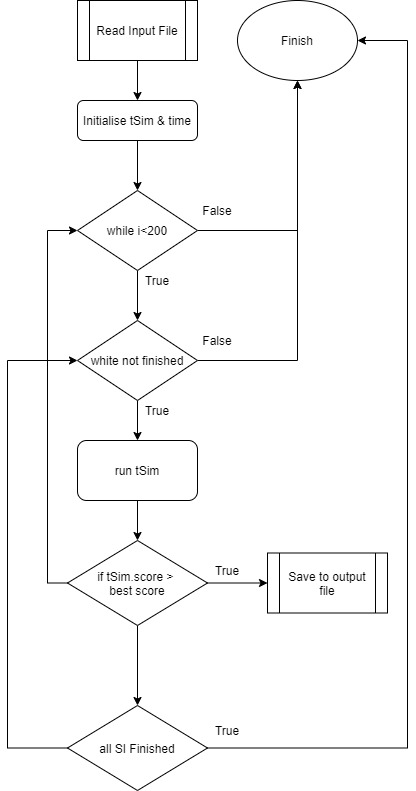
\includegraphics[width=\textwidth]{assets/RL/tSim.jpg}
            \end{figure}
        \end{column}
        \begin{column}{0.7\textwidth}
            \begin{figure}
                \centering
                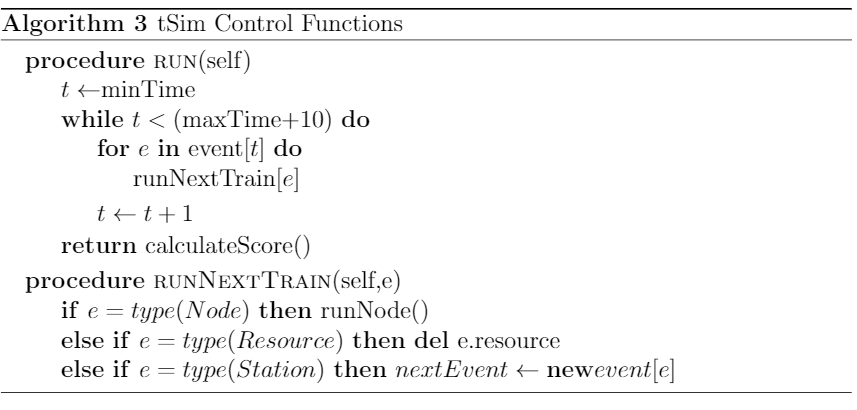
\includegraphics[width=\textwidth]{assets/RL/ALG3.PNG}
            \end{figure}
        \end{column}
    \end{columns}
\end{frame}


\begin{frame}{RL SBB - Reinforcement Learning Applied Algorithm}
    %
    \begin{figure}
        \centering
        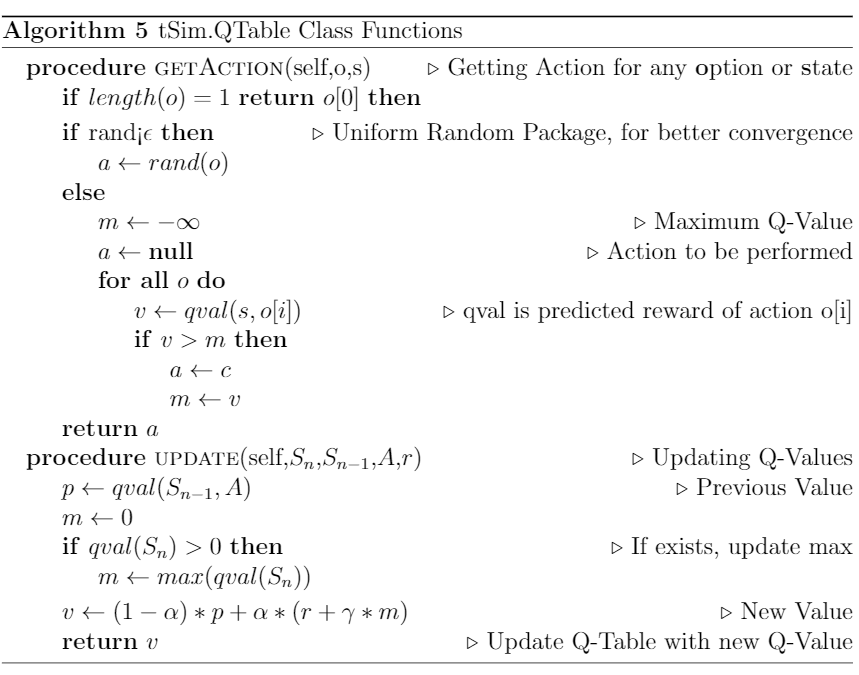
\includegraphics[width=0.55\textwidth]{assets/RL/ALG4.PNG}
    \end{figure}
\end{frame}


\begin{frame}{RL SBB - Results}
    %
    \begin{table}[ht]
        \centering
        \begin{tabular}{|c|cc|cc|cc|}
            \hline
             & \multicolumn{6}{|c|}{\textbf{Solving System}} \\
            \hline
            ID & \multicolumn{2}{|c|}{01} & \multicolumn{2}{|c|}{02} & \multicolumn{2}{|c|}{03}\\
            \hline
             & $ObjVal$ & Time & $ObjVal$ & Time & $ObjVal$ & Time \\
            \hline
            01 & 0 & 5.452 & 0 & 4.296 & 0 & 7.590 \\
            02 & 0.43 & 87 & 0.43 & 72.087 & 0.43 & 77.042 \\ 
            03 & 0.86 & 45 & 0.96 & 198.273 & 0.11 & 200.234 \\ 
            04 & 24.94 & 430 & 24.94 & 439.121 & 024.94 & 435.945 \\ 
            05 & n/a & 1800 & n/a & 1800 & n/a & 1800 \\
            06 & 207.12 & 1355 & 207.12 & 1174.690 & 207.12 & 1750.154 \\ 
            07 & 456.60 & 1800 & 442.33 & 1800 & 467.10 & 1800 \\
            08 & 153.23 & 1800 & 122.70 & 1800 & 233.6 & 1800 \\
            09 & 138.95 & 1800 & 38.25 & 1800 & 43.95 & 1800 \\
            \hline
        \end{tabular}
    \end{table}
\end{frame}


%------------------------------------------------------------------------------------------
% Case Study
\section{Case Study : Manchester}
%------------------------------------------------------------------------------------------

\begin{frame}{Manchester Case Study - Method}
    %
    \begin{columns}[T, onlytextwidth]
        \begin{column}{0.2\textwidth}
            \begin{itemize}
                \item Junction TPH Analysis
                \item Station Timing Data
                \item Previous Case Studies
            \end{itemize}
        \end{column}
        \begin{column}{0.7\textwidth}
            \begin{figure}
                \centering
                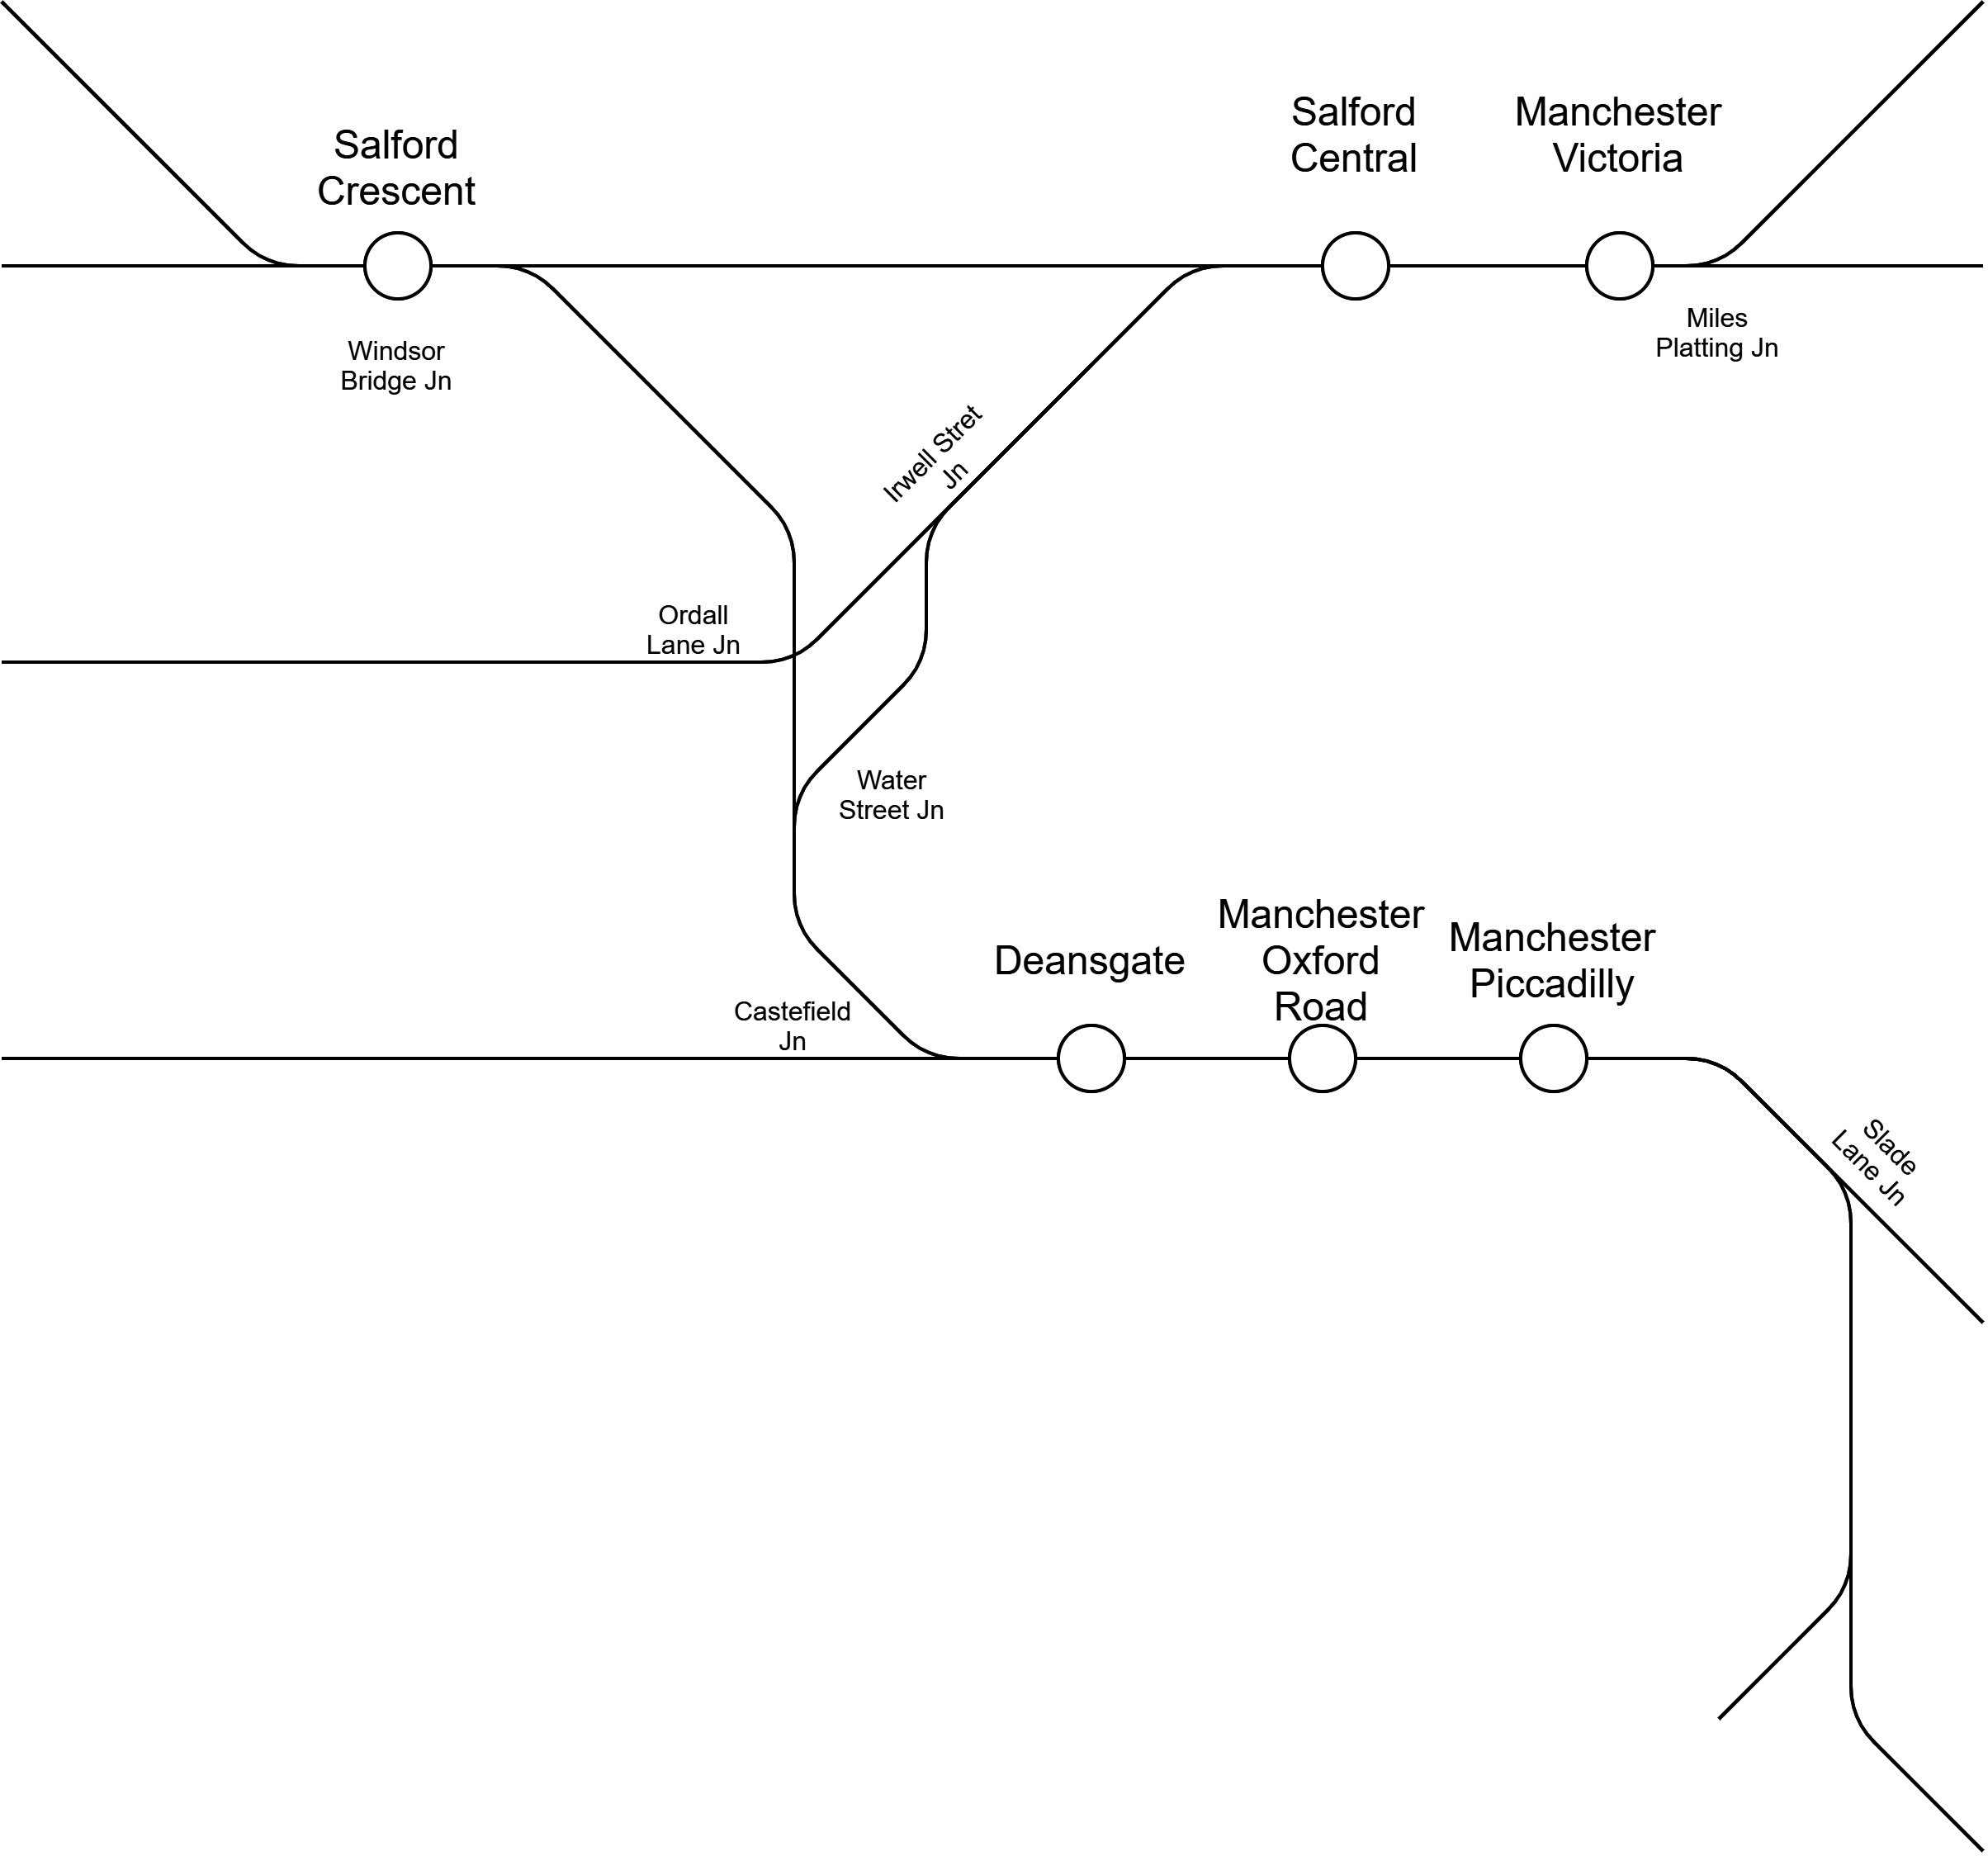
\includegraphics[width=0.65\textwidth]{assets/Case/Geography.jpg}
            \end{figure}
        \end{column}
    \end{columns}
\end{frame}

\begin{frame}{Manchester Case Study - Key Outcomes}
    %
    \begin{figure}
        \centering
        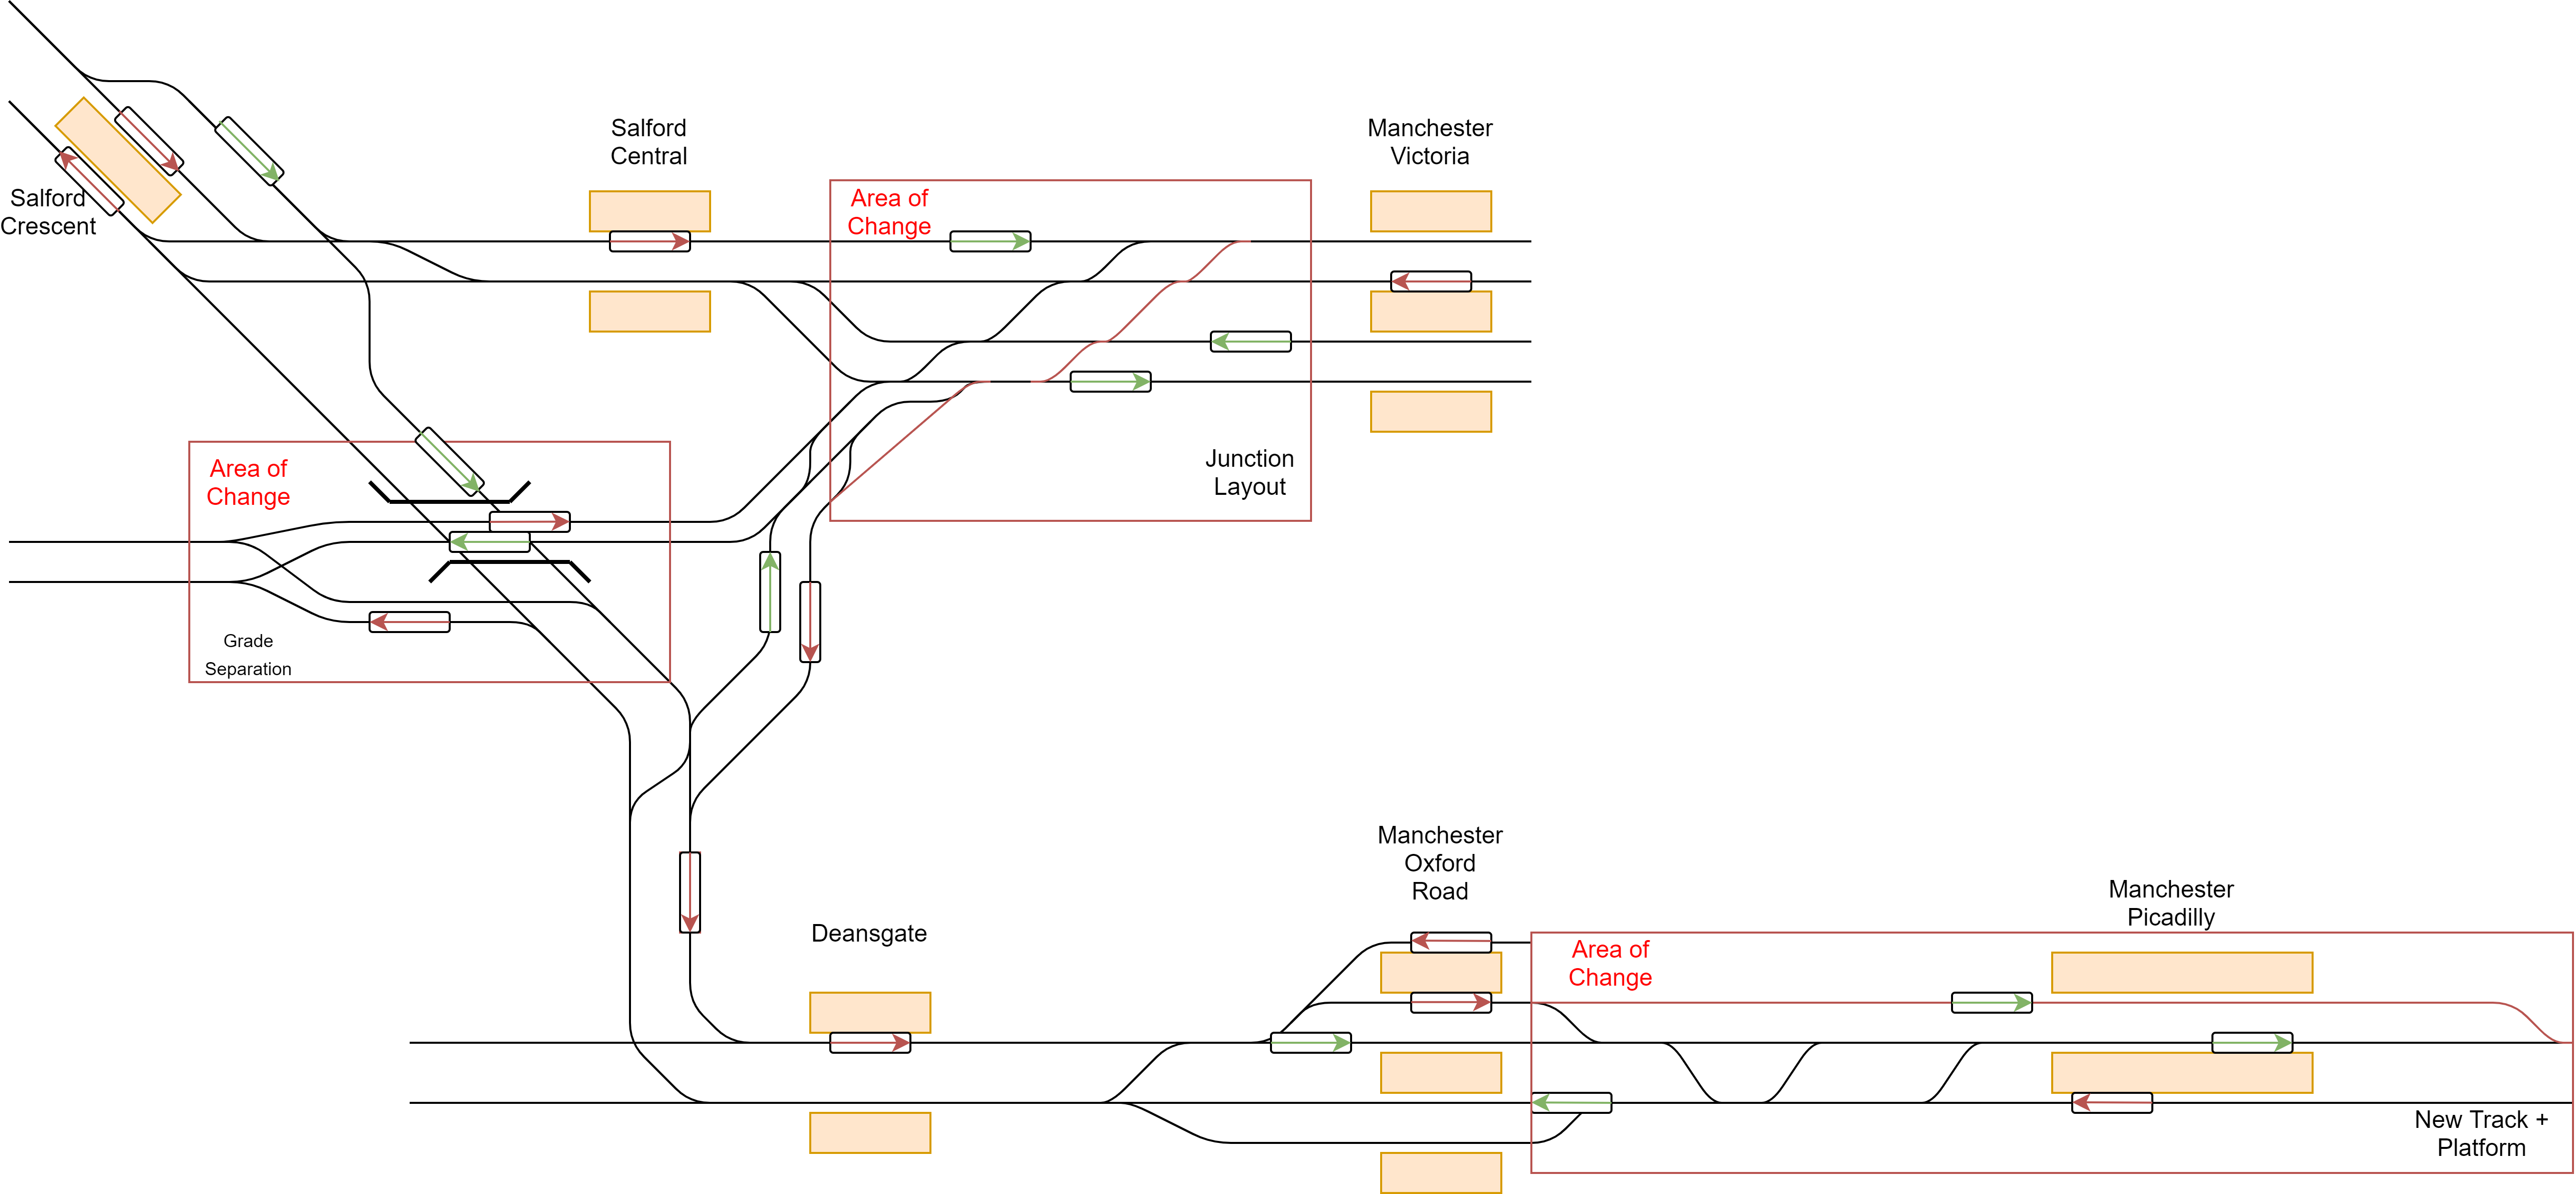
\includegraphics[width=0.9\textwidth]{assets/Case/FullManchester.png}
    \end{figure}
\end{frame}

\begin{frame}{Final Words - Questions}
    %
    Brief Discussion and Q\&A
    \begin{figure}
        \centering
        \begin{subfigure}[t]{0.3\textwidth}
            \centering
            
\includegraphics[width=\linewidth]{assets/.Global/PAPER QRCODE.png}
            \caption{Full Research Paper}
            \label{fig:fw-qr1}
        \end{subfigure}
        \begin{subfigure}[t]{0.3\textwidth}
            \centering
            
\includegraphics[width=\linewidth]{assets/.Global/SLIDES QRCODE.png}
            \caption{Full Slides}
            \label{fig:fw-qr2}
        \end{subfigure}
        \begin{subfigure}[t]{0.3\textwidth}
            \centering
            
\includegraphics[width=\linewidth]{assets/.Global/POSTER QRCODE.png}
            \caption{Full Poster}
            \label{fig:fw-qr3}
        \end{subfigure}
        
    \end{figure}
\end{frame}


\end{document}
